\section{Sekvensdiagrammer}
\subsection{Sekvensdiagram for usecase 1} 
\begin{figure}[H]
	\centering
	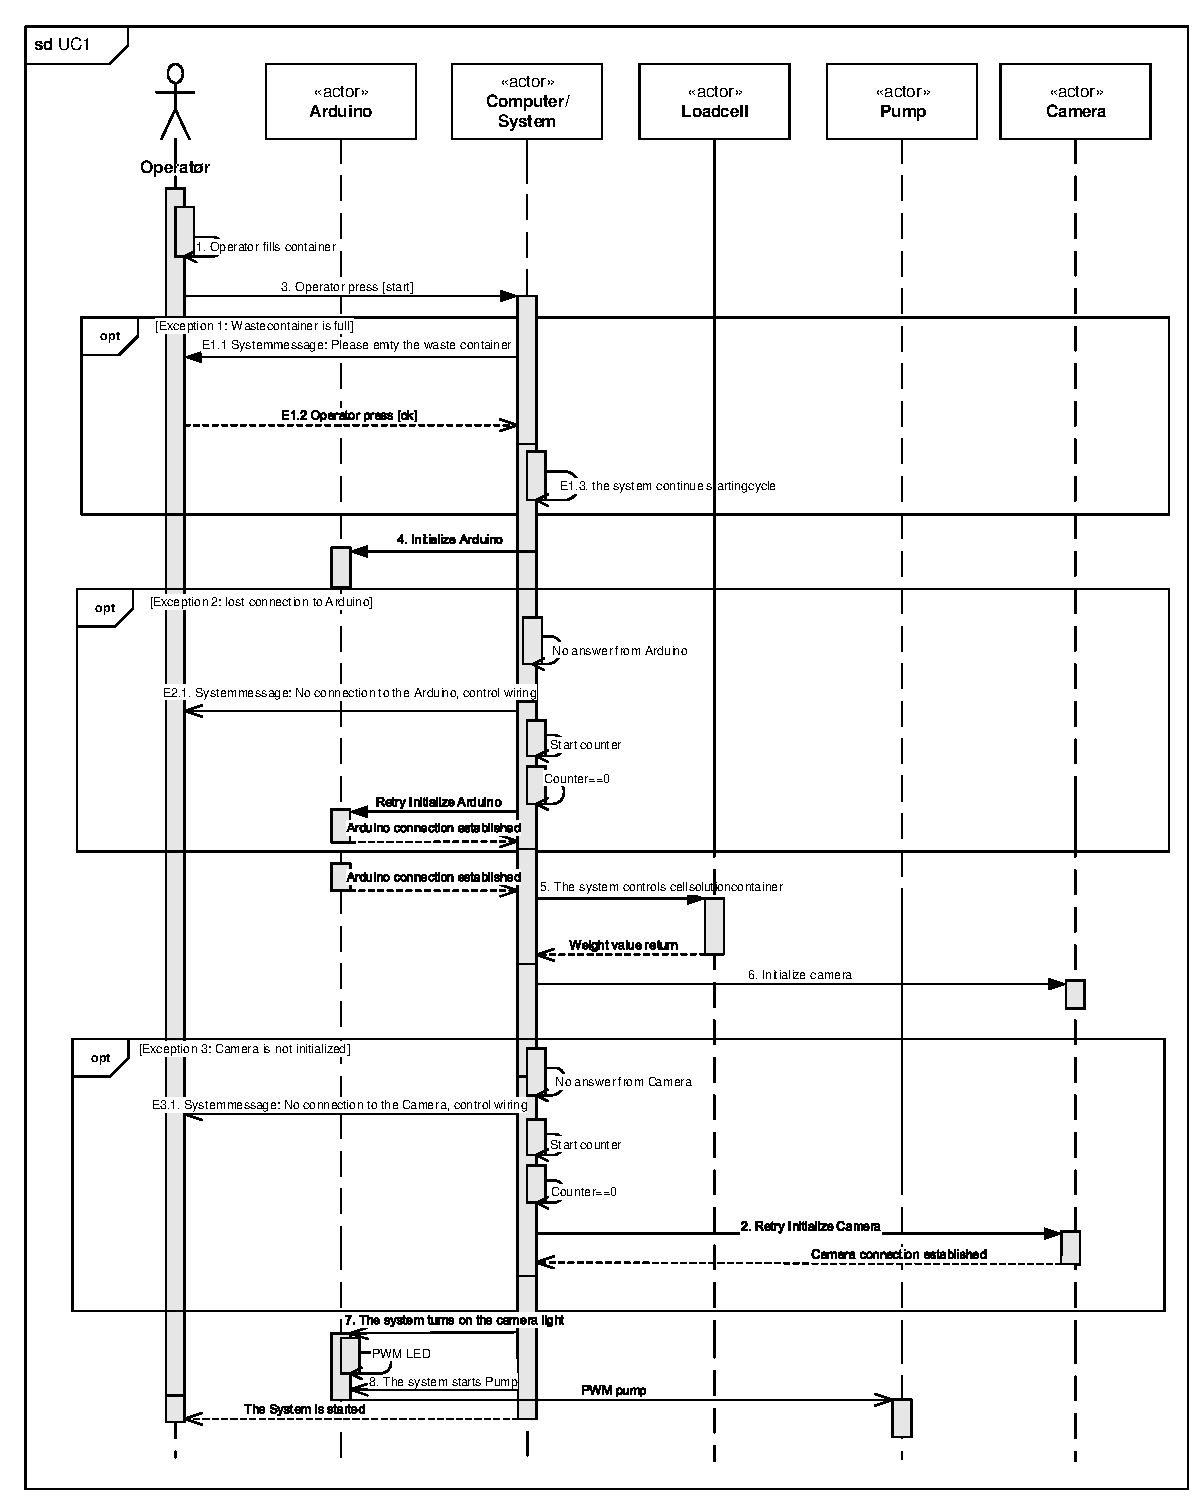
\includegraphics[width=1\textwidth]{pdf/UC1crop.pdf}
	\caption{Sekvensdiagram for usecase 1}
	\label{fig:uc1}
\end{figure}

\subsection{Sekvensdiagram for usecase 2} 
\begin{figure}[H]
	\centering
	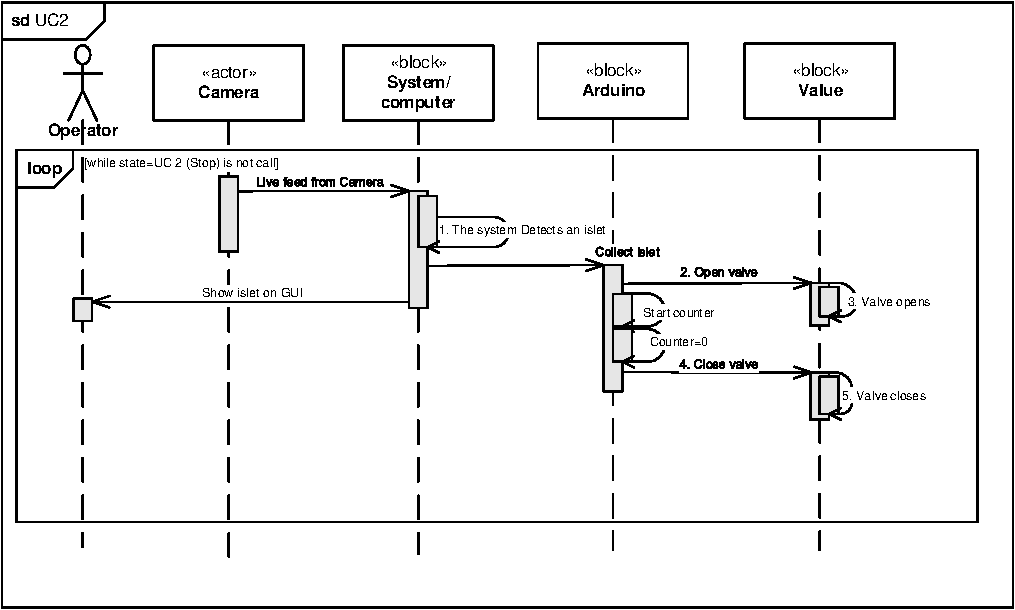
\includegraphics[width=1\textwidth]{pdf/UC2_cropped.pdf}
	\caption{Sekvensdiagram for usecase 2}
	\label{fig:uc1}
\end{figure}

\subsection{Sekvensdiagram for usecase 3} 
\begin{figure}[H]
	\centering
	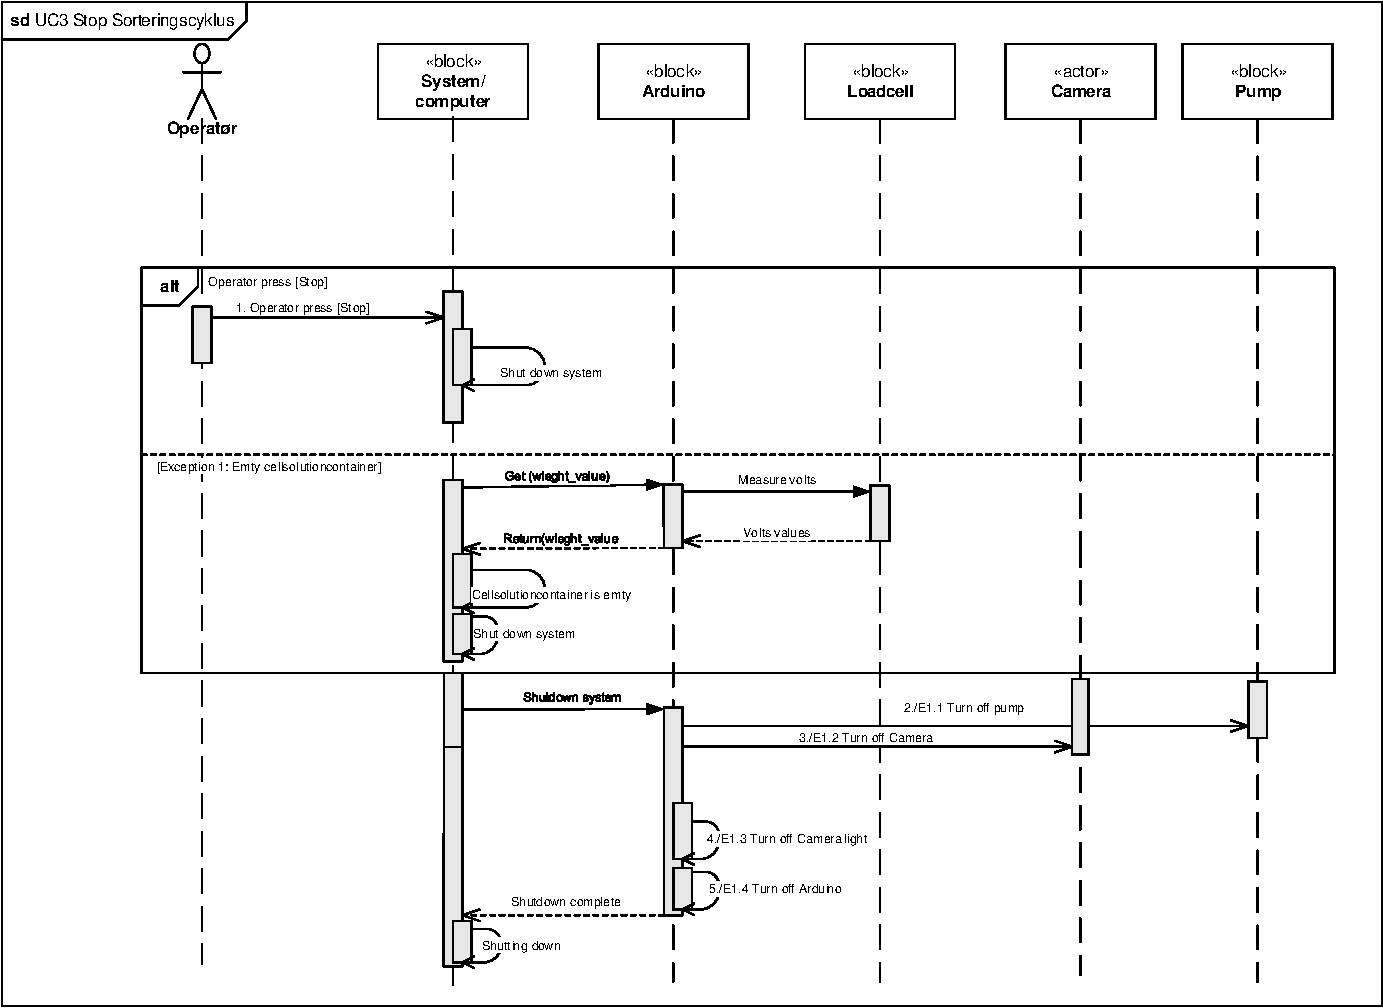
\includegraphics[width=1\textwidth]{pdf/UC3_cropped.pdf}
	\caption{Sekvensdiagram for usecase 3}
	\label{fig:uc1}
\end{figure}

\subsection{Sekvensdiagram for usecase 4} 
\begin{figure}[H]
	\centering
	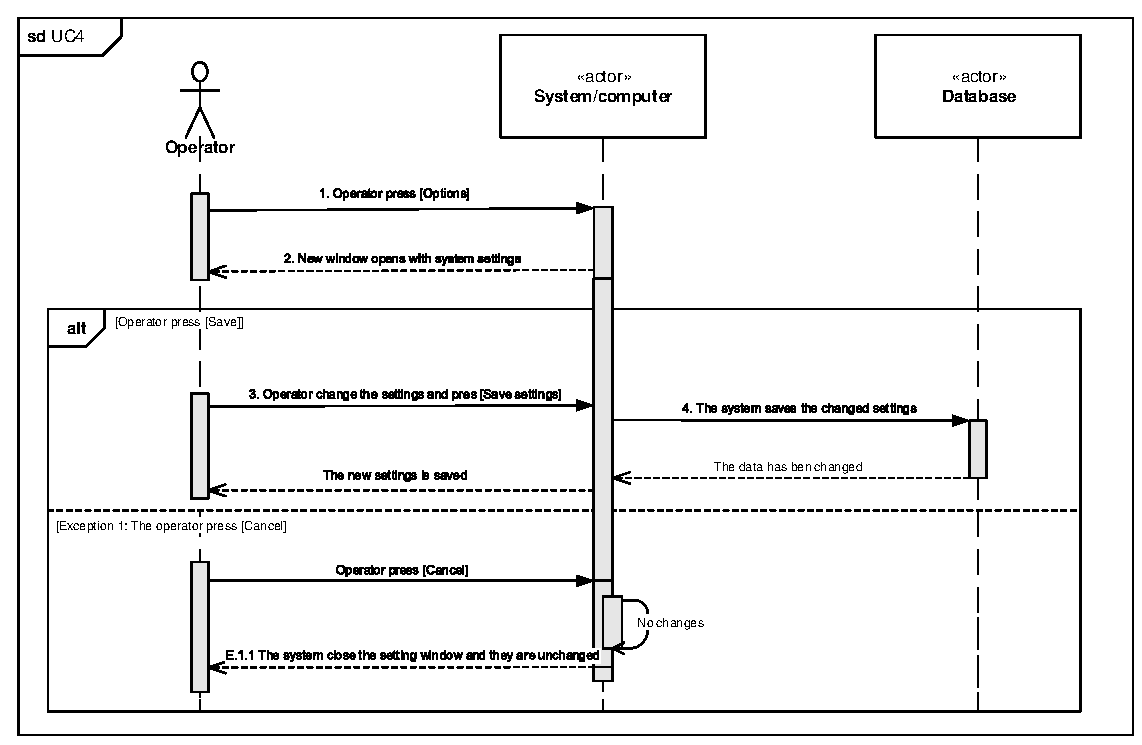
\includegraphics[width=1\textwidth]{pdf/UC4_cropped.pdf}
	\caption{Sekvensdiagram for usecase 4}
	\label{fig:uc1}
\end{figure}

\subsection{Sekvensdiagram for usecase 5} 
\begin{figure}[H]
	\centering
	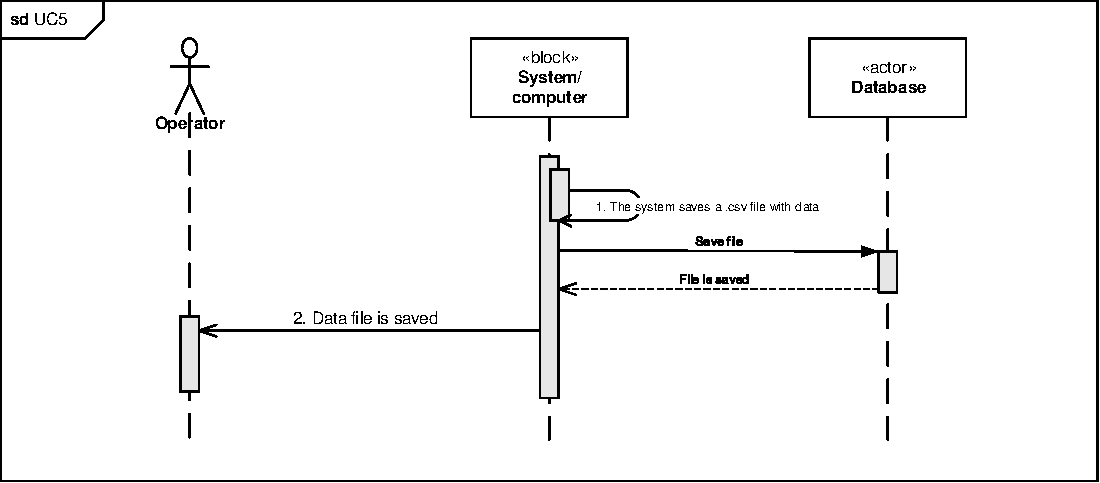
\includegraphics[width=1\textwidth]{pdf/UC5_cropped}
	\caption{Sekvensdiagram for usecase 5}
	\label{fig:uc1}
\end{figure}
